\chapter{THIẾT KẾ BỘ ĐIỀU KHIỂN PID}
    \hspace*{0.6cm}Tiêu chí thiết kế:
    \begin{itemize}
        \item Settling time: $T_s < 1\text{s}$
        \item Overshoot: \%OS < 10\%
    \end{itemize}

    Đối với hệ thống bậc 2, ta có:

    \[
    T_s = \frac{4}{\omega_n}, \quad \%OS = 100e^{\left(-\zeta\pi / \sqrt{1-\zeta^2}\right)}
    \]

    Hệ số giảm chấn $\zeta$ tính từ \%OS:

    \[
    \zeta = \frac{-\ln\left(\frac{\%OS}{100}\right)}{\sqrt{\pi^2 + \ln^2\left(\frac{\%OS}{100}\right)}} = 0.5911
    \]

    Chọn $\zeta = 0.7$

    Suy ra:

    \[
    \omega_n > \frac{4}{\zeta T_s} = \frac{4}{0.7 \cdot 1} = 5.7143
    \]

    Chọn $\omega_n = 8 \text{ (rad/s)}$

    Cực đặc trưng mong muốn là:

    \[
    s_{1,2} = -5.6 \pm 5.713i
    \]

    Hàm truyền closed-loop chuẩn để đạt được tiêu chí thiết kế:

    \[
    G_m(s) = \frac{\omega_n^2}{s^2 + 2\zeta\omega_n s + \omega_n^2} = \frac{64}{s^2 + 11.2s + 64}
    \]

    Phương trình đặc tính của hệ sau khi điều khiển và hồi tiếp để thỏa mãn có 2 cực đặc trưng mong muốn:

    \[
    s^2 + 11.2s + 64
    \]

    Bộ điều khiển PD có dạng:

    \[
    PD(s) = K_p + K_d s
    \]

    Hàm truyền cho vòng kín:

    \[
    T = \frac{PD(s)G(s)}{1 + PD(s)G(s)} = \frac{(K_p + K_d s)G(s)}{1 + (K_p + K_d s)G(s)}
    \]

    Phương trình đặc tính của hệ sau khi điều chỉnh:

    \[
    1 + PD(s)G(s) = 1 + (K_p + K_d s)G(s) = 0
    \]

    \[
    \Leftrightarrow 1 + (K_p + K_d s) \cdot \frac{4.85}{s^2 + 53.51} = 0
    \]

    \[
    \Rightarrow 1 + \frac{(K_p + K_d s) \cdot 4.85}{s^2 + 53.51} = 0
    \]
    \[
    \Leftrightarrow s^2 + 4.85K_d s + 53.51 + 4.85K_p = 0
    \]

    So sánh hệ số với phương trình đặc tính mong muốn, có hệ phương trình:

    \[
    \begin{cases}
    4.85K_d = 11.2 \\
    53.51 + 4.85K_p = 64
    \end{cases}
    \Rightarrow
    \begin{cases}
    K_d = 2.31 \\
    K_p = 2.163
    \end{cases}
    \]

    \textbf{Kiểm tra đáp ứng của hệ sau khi thiết kế bộ PD và hồi tiếp}

    \begin{figure}[H]
        \centering
        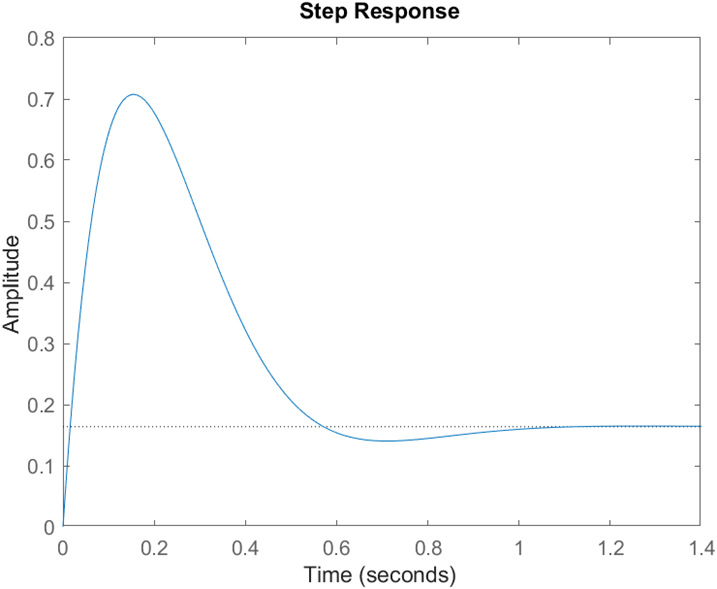
\includegraphics[width=0.7\textwidth]{pictures/PD.png} % Giả sử bạn có ảnh .png
        \caption{Đáp ứng bậc thang của hệ sau khi thiết kế bộ PD}
    \end{figure}

    \begin{itemize}
        \item \textbf{Nhận xét:} Đối với đáp ứng bậc thang, sai số xác lập còn khá lớn, do đó cần thiết kế bộ điều khiển PID để giảm sai số xác lập.
    \end{itemize}

    Khi thiết kế bộ điều khiển PID, phương trình đặc trưng trở thành bậc 3, do đó chọn 1 cực có $s = z$, nằm xa 2 cực mong muốn để ít ảnh hưởng đến hệ, ở đây chọn $z = -12$.

    Phương trình đặc trưng của hệ để có 2 cực mong muốn:

    \[
    (s + 12)(s^2 + 11.2s + 64) = s^3 + 23.2s^2 + 198.4s + 768
    \]

    Bộ điều khiển PID có dạng:

    \[
    PD(s) = K_p + \frac{K_i}{s} + K_d s = \frac{K_d s^2 + K_p s + K_i}{s}
    \]

    \textbf{Hàm truyền cho vòng kín:}
    \[
    T = \frac{PID(s)G(s)}{1 + PID(s)G(s)}
    \]

    Phương trình đặc tính của hệ sau khi điều chỉnh:

    \[
    1 + PID(s)G(s) = 0
    \]

    \[
    \Leftrightarrow s^3 + 4.85K_d s^2 + (53.51 + 4.85K_p)s + 4.85K_i = 0
    \]

    So sánh hệ số với phương trình đặc tính mong muốn, có hệ phương trình:

    \[
    \begin{cases}
    4.85K_d = 23.2 \\
    53.51 + 4.85K_p = 198.4 \\
    4.85K_i = 768
    \end{cases}
    \Rightarrow
    \begin{cases}
    K_p = 29.79 \\
    K_d = 4.7835 \\
    K_i = 158.35
    \end{cases}
    \]

    \textbf{Kiểm tra đáp ứng của hệ sau khi thiết kế bộ PID và hồi tiếp}

    \begin{figure}[H]
        \centering
        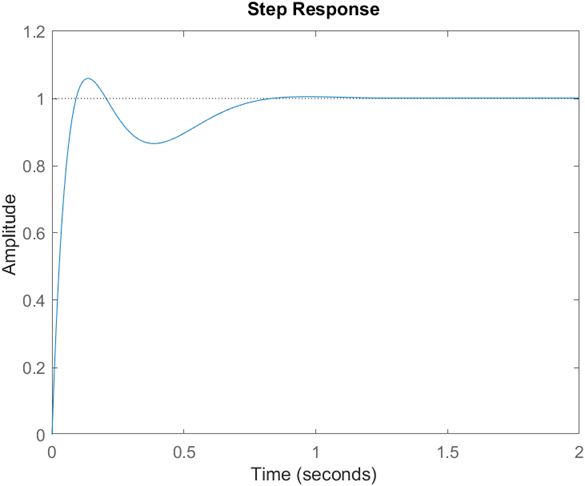
\includegraphics[width=0.7\textwidth]{pictures/PID.png} % ảnh minh họa
        \caption{Đáp ứng bậc thang của hệ sau khi thiết kế bộ PID}
    \end{figure}
    \begin{figure}[H]
        \centering
        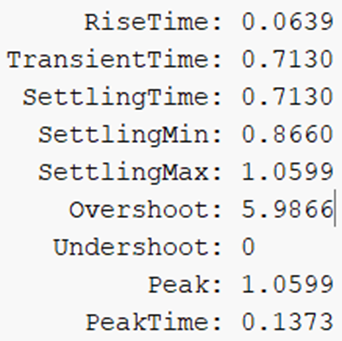
\includegraphics[width=0.5\textwidth]{pictures/specification.png} % ảnh minh họa
        \caption{Thông số đáp ứng bậc thang của hệ sau khi thiết kế bộ PID}
    \end{figure}

